\section{Interpretation}
\label{sec:vergleich}
Die Ergebnisse verdeutlichen, dass die Servicequalität einen starken Einfluss auf die Nutzerzufriedenheit und die Nutzerzufriedenheit wiederum einen starken Einfluss auf den Net Benefit haben (H2 und H4 bestätigt). Der Systemqualität konnte hingegen kein signifikanten Einfluss auf die Nutzerzufriedenheit attestiert werden, ebenso wie der Servicequalität kein direkter Einfluss auf den Net Benefit nachgewiesen werden konnte (H1 und H3 nicht bestätigt). Die Servicequalität verfügt allerdings über einen indirekten Einfluss auf den Net Benefit (Servicequalität --> Nutzerzufriedenheit --> Net Benefit). Besonders der nicht signifikante Einfluss der Systemqualität ist überraschend, zumal die Systemqualität in vergangenen e-learning Studien ein ausschlaggebender Einfluss zugesprochen wurde (Quellen).
Die R$^2$ sind allerdings lediglich im "`mittelguten"' Bereich \parencite[vgl.][S.323]{chin1998partial}. Dies ist ein Zeichen, dass es womöglich noch andere Faktoren gibt, die die Variablen Nutzerzufriedenheit und Net Benefit beschreiben könnten \parencite[vgl.][S.179]{freeze2010success}.  
Als Beispiel 
The COI model (Garrison, Anderson and Archer, 2000) is a three component model that includes a cognitive, social and teaching presence that results in the final educational experience.
Das TAM-Modell fokussiert sich auf die Eigenschaften der Teilnehmer  eines 

Limitationen und Ausblick
Zwar konnte der Systemqualität kein signifikanter Einfluss in dieser Studie nachgewiesen werden, allerdings sollte in zukünftigen Studien nicht auf diesen Faktor verzichtet werden. Obwohl alle Gütekriterien erfüllt wurden, könnte eine größere Stichprobe dem Faktor auch eine größere Bedeutung zumessen. ... hat beobachtet, dass eine Stichprobe ab 200 den Testfehler maßgeblich reduziert bzw. die Genauigkeit der Pfadkoeffizienten erhöht.
Per Definition handelt es sich bei dem analysierten Online Kurs um einen Mentored Open Online Course, inwiefern er sich von einem Massive Open Online Course unterscheidet bedarf einer weiteren Forschung. 
Nichtsdestotrotz sollten weitere Aspekte im Modell Berücksichtigung finden, wie z.B. menschliche Faktoren, inhaltliche Aspekte oder die Arbeitsweise (Teamarbeit, Einzelarbeit). Dies würde dem IS Success Modell weitere Perspektiven eröffnen, wie  in das Modell integriert werden um die Aussagekraft zu erhöhen. M der Nutzer (Selbstdisziplin), Inhalt des MOOCs, Arbeitsweise im MOOC (Team, Alleine) könnten weitere Faktoren darstellen, die den Erfolg eines MOOCs beeinflussen. 
Eine weitere Möglichkeit wäre die Analyse eines MOOCs aus einer anderen Perspektive. Aus der Perspektive von Universitäten oder Unternehmen als Anbieter von MOOCS, sind möglicherweise Kriterien wie Abschlussquote, Gewinn von Mitarbeitern oder Studierende für andere Kurse etc. 


Samplegröße
Limitation der Konstrukte

Ausblick
Ergänzung 
Charakter ebenfalls Analysen (TAM-Modell)



  hingegen nicht bestätigt werden. Die Systemqualität konnte dagegen kein signifikanter Einfluss auf die Nutzerzufriedenheit attestiert werden. Au 
\todo consistency at large. 
Hohe Dropout Raten bei MOOCS. Besonderheiten von MOOC auflisten: 


The story of MOOCs is not going to be told with conventional statistics borrowed from brick-and-mortar classroom models. Rather, our research describes an emerging learning ecosystem, one where enrollment can be casual and nonbinding, learning happens asynchronously, and registrants come from all countries in the world, with diverse intentions and patterns of learning. The metrics we choose should respect their intentions and encourage their learning.\parencite{reich2014tricky}


\begin{figure}[h]
\centering
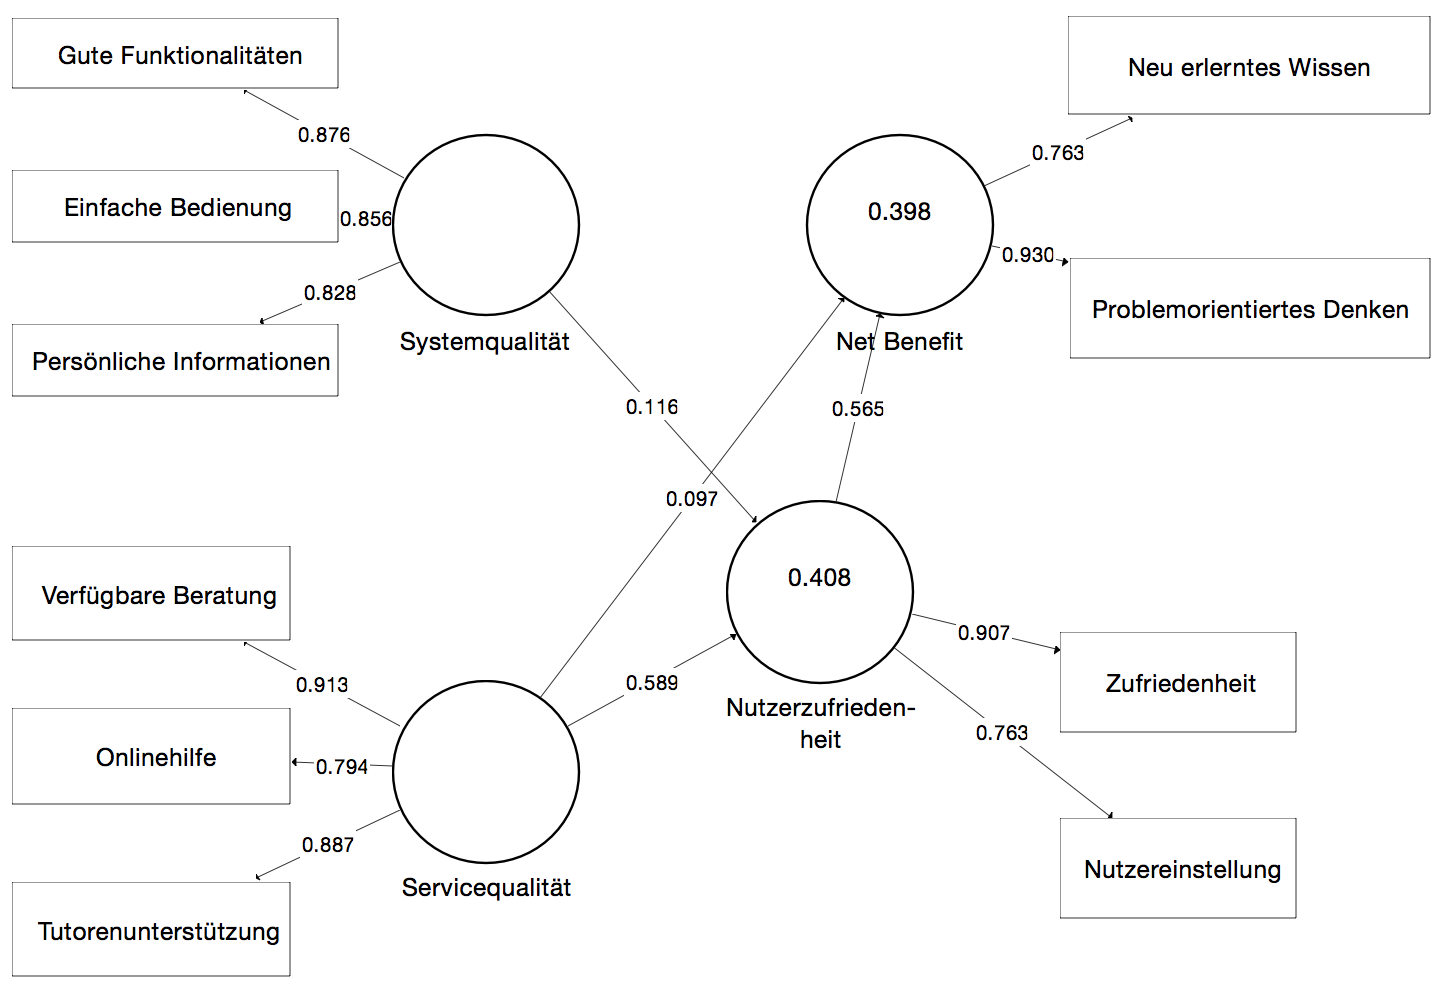
\includegraphics[width=1\textwidth]{Grafiken/pls_bw_3.png}
\caption{PLS Modellergebnisse}
\label{PLS Modellergebnisse}
\end{figure}